%%%%%%%%%%%%%%%%%%%%%%%%%%%%%%%%%%%%%%%%%
% UHCL Computer Architecture Final Project
% Laboratory Report
%
% Original author:
% Mike Moore
%
%%%%%%%%%%%%%%%%%%%%%%%%%%%%%%%%%%%%%%%%%

%----------------------------------------------------------------------------------------
%  PACKAGES AND DOCUMENT CONFIGURATIONS
%----------------------------------------------------------------------------------------

\documentclass{article}

\usepackage{mathtools}
\usepackage{graphicx} % Required for the inclusion of images
\usepackage{listings}
\usepackage{courier}
\usepackage{color}
\usepackage{caption}
\usepackage{graphics}

% Settings for the VHDL Code Listings.

\definecolor{javared}{rgb}{0.6,0,0} % for strings
\definecolor{javagreen}{rgb}{0.25,0.5,0.35} % comments
\definecolor{javapurple}{rgb}{0.5,0,0.35} % keywords
\definecolor{javadocblue}{rgb}{0.25,0.35,0.75} % javadoc
 
\lstset{
      basicstyle=\footnotesize\ttfamily, % Standardschrift
      %numbers=left,               % Ort der Zeilennummern
      numberstyle=\tiny,          % Stil der Zeilennummern
      %stepnumber=2,               % Abstand zwischen den Zeilennummern
      numbersep=5pt,              % Abstand der Nummern zum Text
      tabsize=2,                  % Groesse von Tabs
      extendedchars=true,         %
      breaklines=true,            % Zeilen werden Umgebrochen
      keywordstyle=\color{red},
      frame=b,         
%        keywordstyle=[1]\textbf,    % Stil der Keywords
%        keywordstyle=[2]\textbf,    %
%        keywordstyle=[3]\textbf,    %
%        keywordstyle=[4]\textbf,   \sqrt{\sqrt{}} %
      stringstyle=\color{white}\ttfamily, % Farbe der String
      showspaces=false,           % Leerzeichen anzeigen ?
      showtabs=false,             % Tabs anzeigen ?
      xleftmargin=17pt,
      framexleftmargin=17pt,
      framexrightmargin=5pt,
      framexbottommargin=4pt,
      %backgroundcolor=\color{lightgray},
      showstringspaces=false      % Leerzeichen in Strings anzeigen ?        
 }
 \lstloadlanguages{% Check Dokumentation for further languages ...
         VHDL
 }
\lstset{language=VHDL,
basicstyle=\ttfamily,
keywordstyle=\color{javapurple}\bfseries,
stringstyle=\color{javared},
commentstyle=\color{javagreen},
morecomment=[s][\color{javadocblue}]{/**}{*/},
stepnumber=1,
numbersep=3pt,
tabsize=2,
showspaces=false,
showstringspaces=false}

% Captions for VHDL Code Snippets
\DeclareCaptionFont{blue}{\color{blue}} 

% Captions for VHDL Code Snippets
%\DeclareCaptionFont{blue}{\color{blue}} 

%\captionsetup[lstlisting]{singlelinecheck=false, labelfont={blue}, textfont={blue}}
\usepackage{caption}
\DeclareCaptionFont{white}{\color{white}}
\DeclareCaptionFormat{listing}{\colorbox[cmyk]{0.43, 0.35, 0.35,0.01}{\parbox{\textwidth}{\hspace{15pt}#1#2#3}}}
\captionsetup[lstlisting]{format=listing,labelfont=white,textfont=white, singlelinecheck=false, margin=0pt, font={bf,footnotesize}}


\setlength\parindent{0pt} % Removes all indentation from paragraphs

\renewcommand{\labelenumi}{\alph{enumi}.} % Make numbering in the enumerate environment by letter rather than number (e.g. section 6)

%----------------------------------------------------------------------------------------
%  DOCUMENT INFORMATION
%----------------------------------------------------------------------------------------

\title{Homework 1 \\ CENG 5131} % Title

\author{Mike \textsc{Moore}} % Author name

\date{\today} % Date for the report

\begin{document}

\maketitle % Insert the title, author and date

\begin{center}
\begin{tabular}{l r}
Instructor: & Dr. Thomas Harman % Instructor/supervisor
\end{tabular}
\end{center}




\newpage

%----------------------------------------------------------------------------------------
%  Problem 1
%----------------------------------------------------------------------------------------

%%%%%%%%%%%%%%%%%%%%%%%%%%%%%%%%%%%%%%%%%%%%%%%%%%%%%%%%%%%%
\section{Problem 1}

An Arithmetic Logic Unit (ALU) is a fundamental component within the central processing
unit (CPU). It is responsible for both the arithmetic and logical operations of the CPU,
and as such, it is responsible for a large part of the CPU work load. Modern ALU designs
can be quite complex, and often they are not actually a single unit within the CPU. For 
simplicity, this report focuses on a simplified four bit ALU design.

%----------------------------------------------------------------------------------------
%  SECTION 1
%----------------------------------------------------------------------------------------

%%%%%%%%%%%%%%%%%%%%%%%%%%%%%%%%%%%%%%%%%%%%%%%%%%%%%%%%%%%%
\section{Part A}
\subsection{Problem Statement}
Compute the radian frequency ω and the period T in seconds of the
sinewave:




The ALU was designed to meet the following list of requirements:

\begin{itemize}
   \item The unit has two 4-bit inputs, register A and register B. 
   \item The unit must be able to add, increment, decrement, transfer and also perform basic logic operations AND, OR, NOT, XOR. 
   \item The unit will have 4-bit select line called Operation Select, which would direct the unit as to which operation to perform. 
   \item In addition the unit must also be able to do shift operations (right shift, left shift etc). 
   \item The unit has a Carry-in and also has Carry-out. 
\end{itemize}

We see from the above requirements list that we will need to design an ALU that has a total of thirteen
input bits. Eight will be used for the two four bit operand registers, and another four will be used for
the op-code. Finally, a single carry in bit is also required. The outputs are a little bit simpler. We will only need four bits for the data out, and a single bit for the carry out.

\newpage

I'm not ready to open source it. The current state of the code is atrocious. I will fix that in time. However, I am willing to provide access to the repository I store it in for anyone that can help in the development. I personally feel like there's a small niche for open-source 3d quad simulations that allow you to plug and play your own control code. If anyone is interested in helping with something like that, PM me. Let's talk about it!

That's a good question. I have a few ideas on that one. 

Right now, in the real system, the "controller code" is simply an algorithm written in C and then compiled on a micro-controller. In this simulation, I just make sure to preserve the same inputs/outputs, and then put in the same control algorithm (a function call).

My longer term idea is to use this simulation in a "hardware in the loop" fashion. This is where I directly connect up the simulation to the real quadcopter's communications system. It would go something like this real quad -> wireless channel -> communications web server -> tcp connection to simulator. 

Following that route, you could disable the dynamics model running on the simulator, and simply update the scene with real data from the quad. This would allow a pathway to have simulated control systems operating on live data. You would have the possibility of, in real-time, analyzing the difference between a new simulated control system vs the current design of the control system running on the real quad. That would be just one application.

I really want to write a controller that is capable of flying pre-defined trajectory's (GPS co-ords). I'm pretty sure this sim is going to make that task much, much easier.







\subsection{ALU Block Diagram}
With this understanding of our requirements, the next step is to depict the ALU in a functional block diagram form. This will later allow for us to more easily translate the preliminary design to a VHDL module. The block diagram description of our ALU is provided below. Note how the inputs and outputs directly map to statements in the list of requirements.
\begin{figure}[ht!]
\centering
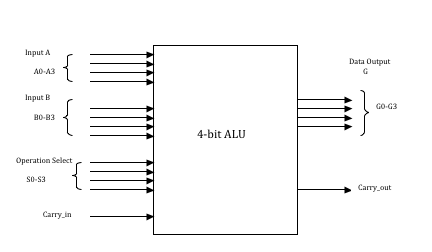
\includegraphics[width=100mm, height=50mm]{images/BlockDiagramALU.png}
\caption{Four Bit ALU Block Diagram}
\label{overflow}
\end{figure}

\subsection{ALU Operations}
The required operations for the ALU are listed below.
\begin{figure}[ht!]
\centering
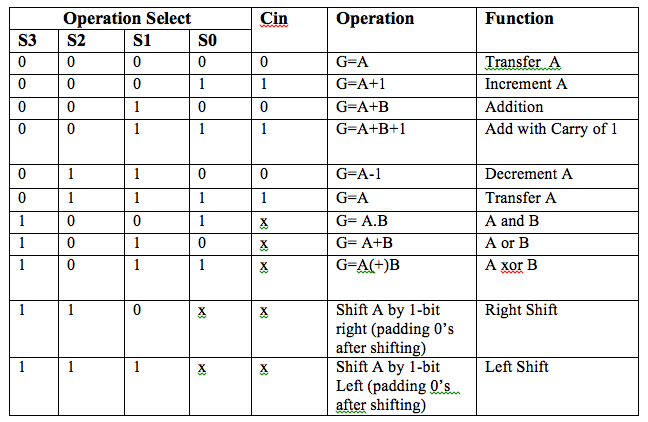
\includegraphics[width=100mm, height=50mm]{images/ALUOps.png}
\caption{Four Bit ALU Required Operations} 
\label{overflow}
\end{figure}

%----------------------------------------------------------------------------------------
%  SECTION 3
%----------------------------------------------------------------------------------------

%%%%%%%%%%%%%%%%%%%%%%%%%%%%%%%%%%%%%%%%%%%%%%%%%%%%%%%%%%%%
\section{The ALU VHDL Module}

The next step in the ALU design process was to actually write out the
VHDL to perform the desired functions. A behavioral model is used to implement
the ALU. This makes the code more readable at the expense of obfuscating the underlying
hardware implementation. A structural model would be more revealing in that case, but for
the sake of code readability and ease of implementation, a behavioral model was decided upon
for this design.
